		\ifx \allfiles \undefined		%编译PPT时注释该行
\documentclass{ctexart}				%编译PPT时注释该行
\usepackage{ifthen}
%\usepackage[a3paper,landscape,showframe,margin=1.25in]{geometry}
%\usepackage[a3paper,landscape,margin=1.1in]{geometry}
\usepackage[a3paper,landscape,top=1.25in,bottom=0.8in,left=1in,right=1in]{geometry}
\usepackage{tikz,units}
\usepackage{circuitikz}
\usepackage{subfig}
\usetikzlibrary{backgrounds,circuits.ee.IEC.relay}
\usetikzlibrary{positioning}
\usepackage{tikzsymbols}
\usepackage{pgffor}
\usetikzlibrary {math}
\usepackage{lastpage}
\usepackage{fancyhdr}
\pagestyle{fancy}
\fancyhf{}
\fancyhead[ER,OL]{\heiti \zihao{-5} 热工专业图纸}
\fancyhead[OR,EL]{\heiti \zihao{-5} \leftmark}
\fancyfoot[CE,CO]{热工专业图纸~第~\thepage~页(共 \pageref{LastPage} 页)}
\renewcommand{\headrulewidth}{0.4pt}
\renewcommand{\footrulewidth}{0.4pt}
\tikzset{
box/.style={rectangle,minimum height=17pt,minimum width=20pt,text=red}
}
\tikzset{
boxA/.style={rectangle,minimum height=17pt,minimum width=20pt,draw=black}
}
\tikzset{
boxB/.style={rectangle,minimum height=17pt,minimum width=30pt,draw=black}
}
\tikzset{
boxC/.style={rectangle,minimum height=17pt,minimum width=120pt,draw=black}
}
\tikzset{
boxD/.style={minimum width=140pt,above left}
}

\lhead{热工专业图纸}
\rhead{锅炉本体吹灰器电气原理图}
\cfoot{热工专业图纸~第~\thepage~页 (共 \pageref{LastPage} 页)}
\begin{document}
		\else						%编译PPT时注释该行
			\chapter{锅炉本体吹灰器电气原理图}	%编译PPT时注释该行
		\newpage
		\fi						%编译PPT时注释该行
\begin{center}
{\huge 锅炉本体吹灰器电气原理图}\\
\end{center}
\begin{center}

	\begin{figure}[h]
\subfloat[动力回路]{
\label{fig:improved_subfig_a}
		\begin{minipage}{300pt}
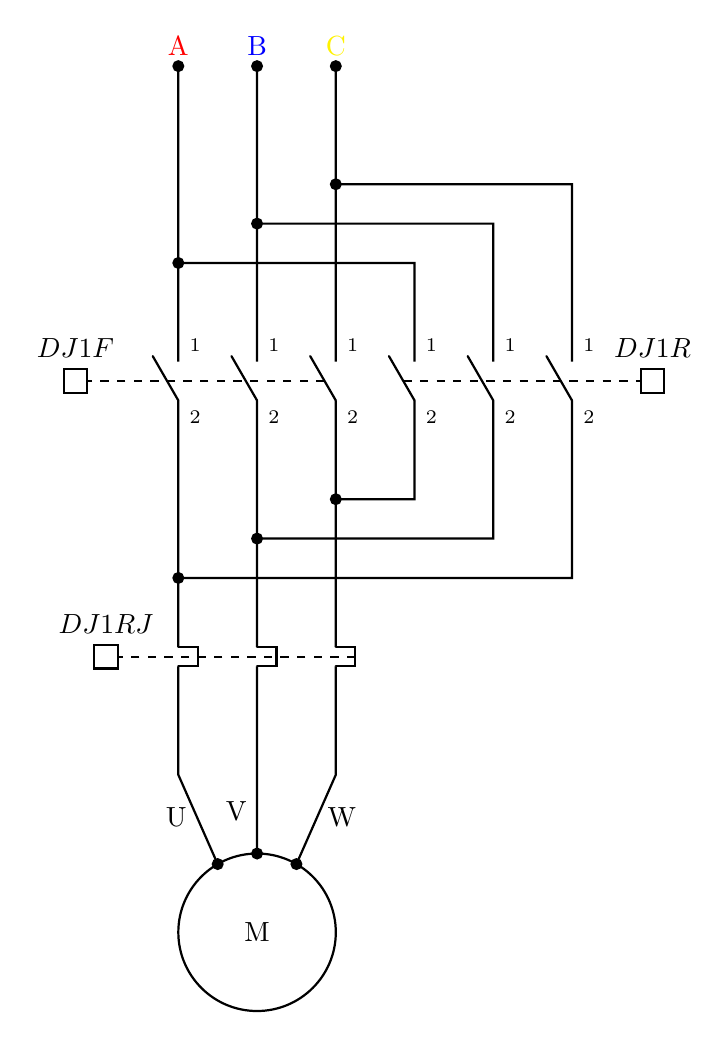
\begin{tikzpicture}[circuit ee IEC relay,thick,scale=1]

%d动力回路
\node (M) at (1,0) {M};%绝对坐标
\coordinate (V1) at (1,2);
\coordinate[right=1 of V1] (W1);
\coordinate[left=1 of V1] (U1);
\draw (M) circle (1);

\draw (M) ++(120:1) node [contact,name=U]{};
\draw (M) ++(90:1) node [contact,name=V]{};
\draw (M) ++(60:1) node [contact,name=W]{};

\draw (V) -- node[left] {V} (V1) -- ++(0,1)
to [thermic sensor] ++(0,1) -- ++(0,1)
node [contact,name=V2]{} -- ++(0,1.5)
to [make contact={term=1,term'=2}] ++(0,1) -- ++(0,1.5)
node [contact,name=V3]{} -- ++(0,2)
node [contact,name=V4]{};
\node[above,blue] at(V4) {B};

\draw (U) -- node[left] {U} (U1) -- ++(0,1)
to [thermic sensor] ++(0,1) -- ++(0,0.5)
node [contact,name=U2]{} -- ++(0,2)
to [make contact={term=1,term'=2}] ++(0,1) -- ++(0,1)
node [contact,name=U3]{} -- ++(0,2.5)
node [contact,name=U4]{};
\node[above,red] at(U4) {A};

\draw (W) -- node[right] {W} (W1) -- ++(0,1)
to [thermic sensor={name=FR}] ++(0,1) -- ++(0,1.5)
node [contact,name=W2]{} -- ++(0,1)
to [make contact={name=KM1,term=1,term'=2}] ++(0,1) -- ++(0,2)
node [contact,name=W3]{} -- ++(0,1.5)
node [contact,name=W4]{};
\node[above,yellow] at(W4) {C};

\draw (V2) -- ++(3,0) -- ++(0,1.5) to [make contact={term=1,term'=2}] ++(0,1) -- ++(0,1.5) -- (V3);

\draw (U2) -- ++(5,0) -- ++(0,2) to [make contact={term=1,term'=2}] ++(0,1) -- ++(0,2) -- (W3);

\draw (W2) -- ++(1,0) -- ++(0,1) to [make contact={name=KM2,term=1,term'=2}] ++(0,1) -- ++(0,1) -- (U3);

\draw[dashed](KM1.mid) -- ++(-3,0) node[left,draw,solid,minimum size=3mm,label={[above]:$DJ1F$}]{};

\draw[dashed](KM2.mid) -- ++(3,0) node[right,draw,solid,minimum size=3mm,label={[above]:$DJ1R$}]{};

\draw[dashed](FR.mid) -- ++(-3,0) node[left,draw,solid,minimum size=3mm,label={[above]:$DJ1RJ$}]{};




	\end{tikzpicture}
		\end{minipage}
}
\subfloat[控制回路]{
\label{fig:improved_subfig_b}
		\begin{minipage}{600pt}
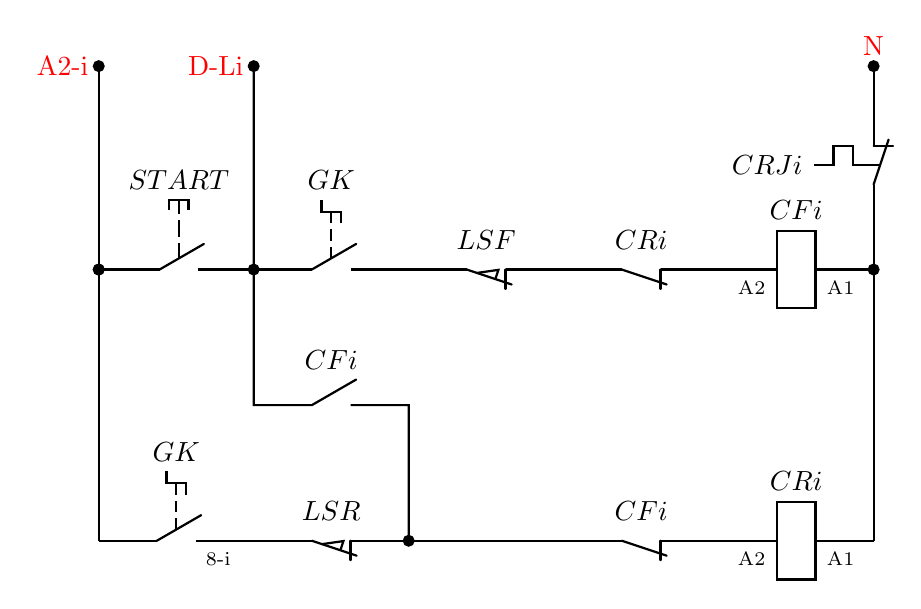
\begin{tikzpicture}[circuit ee IEC relay,thick,x=8\tikzcircuitssizeunit,y=7\tikzcircuitssizeunit]
		
			\draw (0,0) node [shape=coordinate](A1){} -- ++(0,2) node [contact,name=B1]{}
				-- ++(0,1.5)node [contact,name=C1]{} ++(1,0)node [contact,name=C2]{};
		\draw (A1)
		to [make contact={turn switch={info=$GK$},term=8-i}] ++(1,0)
		to [break contact={position switch={info=$LSR$}}] ++(1,0)
		node [contact,name=A2]{} -- ++(1,0)
		to [break contact={info=$CFi$}] ++(1,0)
		to [relay coil={info=$CRi$,term=A1,term'=A2}] ++(1,0) 
		node [shape=coordinate](A3){};

		\draw (B1) node[contact]{}
		to [make contact={push button={info=$START$}}] ++(1,0)
		node [contact,name=B2]{}
		to [make contact={turn switch={info=$GK$}}] ++(1,0)
		to [break contact={position switch={info=$LSF$}}] ++(1,0)
		to [break contact={info=$CRi$}] ++(1,0)
		to [relay coil={info=$CFi$,term=A1,term'=A2}] ++(1,0)
		node [contact,name=B3]{};

		\draw (A3) --(B3) 
		to [break contact={thermal switch={info=$CRJi$}}] ++(0,1.5)node [contact,name=N]{};
		
		\draw (C2) -- (B2) -- ++(0,-1) to [make contact={info=$CFi$}] ++(1,0) -- (A2);
		
\node[above,red] at(N) {N};
\node[left,red] at(C1) {A2-i};
\node[left,red] at(C2) {D-Li};
	\end{tikzpicture}
		\end{minipage}
}
\caption{锅炉本体吹灰器电气回路图}
\label{fig:improved_subfig}
	\end{figure}
	\clearpage
\end{center}
		\ifx \allfiles \undefined
\end{document}

\fi
